\documentclass[12pt]{article}

\usepackage{scicite,times,graphicx,float,hyperref}
\usepackage[skip=0pt]{caption}

\topmargin -1.0cm
\oddsidemargin 0.0cm
\textwidth 16cm 
\textheight 23cm
\footskip 1.0cm

\newenvironment{sciabstract}{%
\begin{quote} \bf}
{\end{quote}}

\newcounter{lastnote}
\newenvironment{scilastnote}{%
  \setcounter{lastnote}{\value{enumiv}}%
  \addtocounter{lastnote}{+1}%
  \begin{list}%
  {\arabic{lastnote}.}
  {\setlength{\leftmargin}{.22in}}
  {\setlength{\labelsep}{.5em}}
}
{\end{list}}

\title{Lab Work 2} 

\author
{André Pedrosa [85098], Filipe Pires [85122], João Alegria [85048]\\
\\
Algorithmic Information Theory\\
\normalsize{Department of Electronics, Telecommunications and Informatics}\\
\normalsize{University of Aveiro}\\
} 

\date{\today{}}

%%%%%%%%%%%%%%%%% END OF PREAMBLE %%%%%%%%%%%%%%%%

\begin{document} 

\baselineskip18pt

\maketitle 

\section*{Introduction}

This report aims to describe the work developed for the second assignment
of the course of 'Algorithmic Information Theory', explaining all programs
developed by us, and presenting the results we considered most relevant 
regarding the quality of the solutions. 

The programs implemented in C++ have the purpose of analysing and encoding
audio files and ultimately being capable of, from a small audio segment, 
identifying the music that it most likely belongs to.

Along with the description of the solution, we also discuss the effects
of the variation of the programs' parameters and how accurate are the results.
All code developed is publicly accessible in our GitHub repository:
\url{https://github.com/joao-alegria/TAI} .
\newpage

\section*{1. Data Visualization}

In this chapter we present a description of the dataset used, the small script 
we developed to convert audio segments from stereo to mono and the histograms
we are capable of plotting by adapting one of the scripts given along with the
assignment's description \cite{trab1}.

\subsection*{1.1. Dataset}

We were given the access to a small dataset containing 7 audio files from 
different musics. It was these music fragments we used to test our code during 
development.
Each audio file is in \texttt{.wav} format and has two signal channels (stereo).
They vary between 13 and 29 seconds of audio and, when played, none seems to 
contain significant noise.

For testing the performance of the programs once the development phase was
completed, we came up with our own dataset of musics of different genres.
These music files vary between 3:07 and 8:09 minutes and have the same format 
and number of channels as the original dataset.
As they were downloaded from the original sources, their quality is close to 
ideal.

\subsection*{1.2. Mono Conversion}

One of the tasks proposed was to create a script that converts stereo audio 
files into mono.
This was fairly straightforward to do, as it only required for us to read the v
alues from all signal channels and calculate the average of each.
The script is executed in the format presented below, once built:

\begingroup
\addtolength\leftmargini{-0.4in}
\begin{quote}
\begin{verbatim}
$ ./wavquant inputFile outputFile [-q quantSize] [-r reductFactor]
\end{verbatim}
\end{quote}
\endgroup

This script, \texttt{wavquant.cpp}, is also used for other purposes, in which 
the \texttt{quantSize} and \texttt{reductFactor} parameters are useful.
For this reason, we made the parameters optional, so that a user can run 
\texttt{wavquant} to simply convert stereo files into mono, with a default 
number of bits used to encode each value of the segment (each sample) of 16 and 
no frequency reduction factor.
This script is mentioned further ahead in greater detail.

\subsection*{1.3. Histograms}

We were also given a script called \texttt{wavhist.cpp} that outputted to the 
terminal the histogram of an audio file.
We adapted this script so that it accepts both stereo and mono audio files 
and plots in a figure the histogram of one of the audio channels with the help of \texttt{gnuplot} \cite{gnuplot}, a portable command-line driven graphing utility. The resulting WAVHist script has the following interface:

\begingroup
\addtolength\leftmargini{-0.4in}
\begin{quote}
\begin{verbatim}
$ ./wavhist <inputFile> <channel>
\end{verbatim}
\end{quote}
\endgroup

Figures \ref{fig:histogram_stereo} and \ref{fig:histogram_mono} contain the 
histograms plotted from the same music in the original format (stereo) and after 
its conversion to mono. 
The x axis represents the frequency of the values and the y axis the number of 
occurences in the music of each frequency.

\begin{figure}[H]
  \centering
  \begin{minipage}{.5\textwidth}
    \centering
    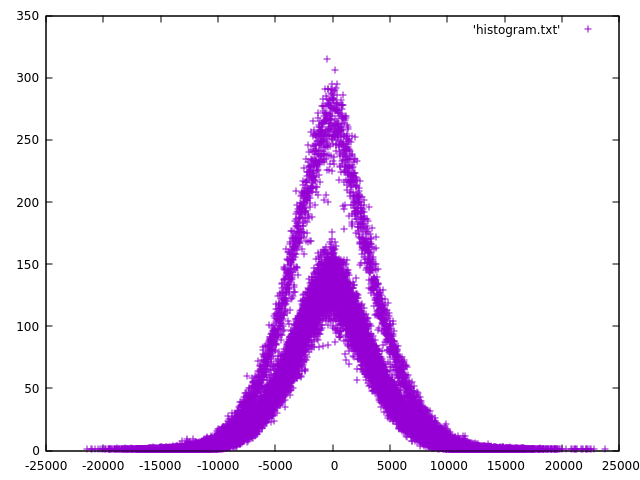
\includegraphics[width=\linewidth]{sample01_stereo_0.png}
  \end{minipage}%
  \begin{minipage}{.5\textwidth}
    \centering
    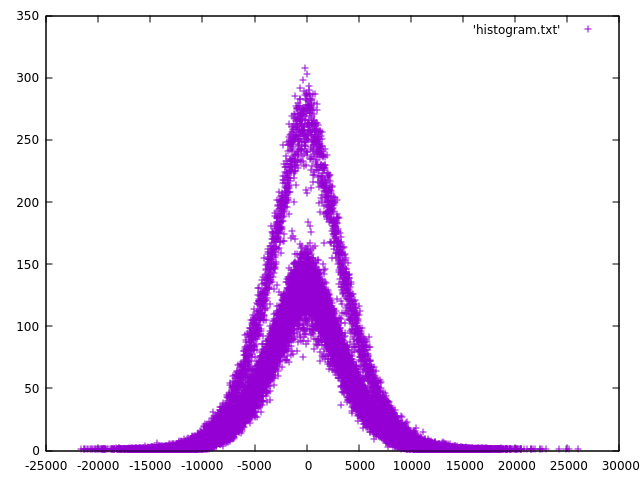
\includegraphics[width=\linewidth]{sample01_stereo_1.png}
  \end{minipage}
  \caption{Histogram of sample01 in the original format - channels 0 and 1.}
  \label{fig:histogram_stereo}
  
  \centering
  \begin{minipage}{.5\textwidth}
    \centering
    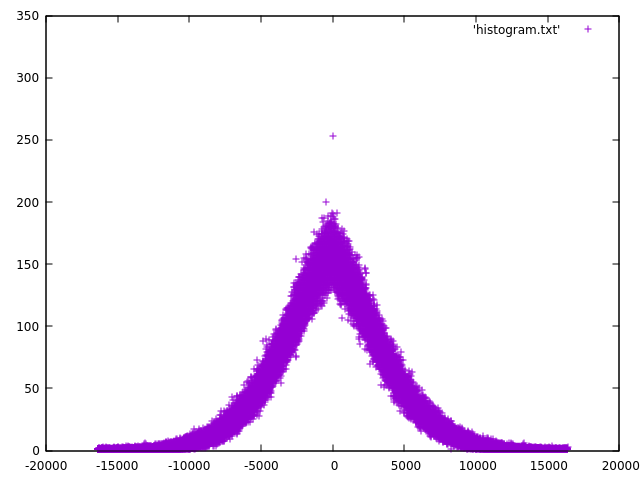
\includegraphics[width=\linewidth]{sample01_16_1.png}
  \end{minipage}%
  \caption{{Histogram of sample01 after its conversion to mono (1 channel only).}}
  \label{fig:histogram_mono}
\end{figure}

It's clearly visible that the mono conversion affected the way the music file was represented maintaining the fidelity to the original song. Analyzing Figures \ref{fig:histogram_stereo} and \ref{fig:histogram_mono} the first first thing we see is the disappearance of the gap represented in both channels of the stereo signal. In the first place, the gap exists because the song has that frequency registry, to note that each value in the x axis as one and only one y value, so to obtain this gap close frequencies have very different counts. When converting to mono is natural that this gap disappear, since to obtain a mono signal from a stereo one, it's necessary to take both left and right sample and obtain the average, obtaining then just ine value where there were two.

Another interesting occurrence observed from the Figures \ref{fig:histogram_stereo} and \ref{fig:histogram_mono} is that in the mono signal, the number of occurrences decrease a little bit. This once again is explained by the mono conversion process, since each two samples will be aggregated in only one, all the frequencies that occur very frequently have a high probability of being pared with another frequency, spreading the frequency counts in a more controlled fashion.

\begin{figure}[H]
  \begin{minipage}{.5\textwidth}
    \centering
    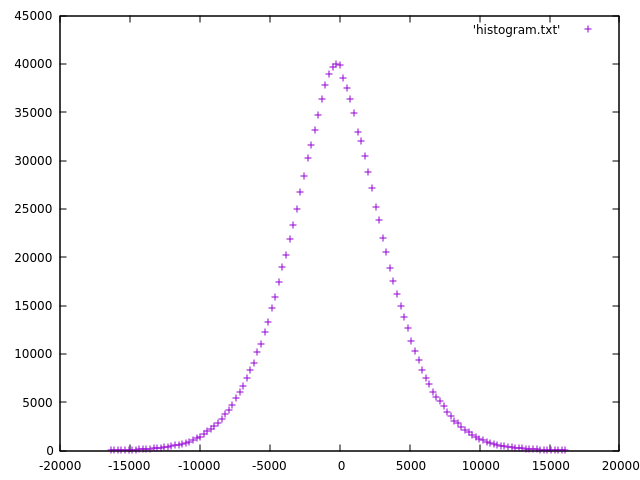
\includegraphics[width=\linewidth]{sample01_8_1.png}
    \caption{{8 bits, no reduction}}
    \label{fig:8_no}
  \end{minipage}
  \begin{minipage}{.5\textwidth}
    \centering
    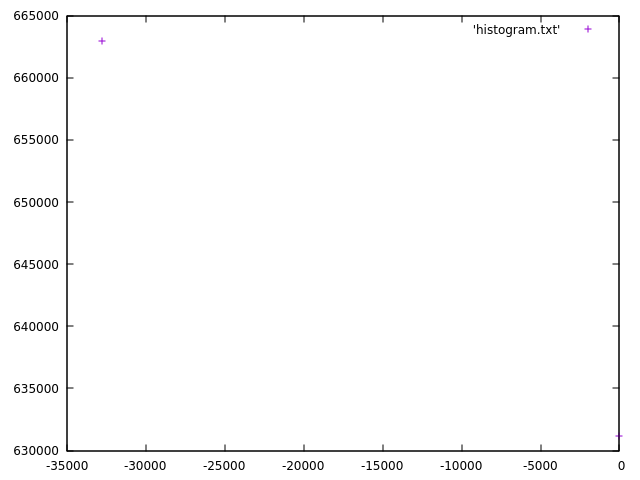
\includegraphics[width=\linewidth]{sample01_1_1.png}
    \caption{{1 bit, no reduction}}
    \label{fig:1_no}
  \end{minipage}
\end{figure}
\begin{figure}[H]
  \begin{minipage}{.5\textwidth}
    \centering
    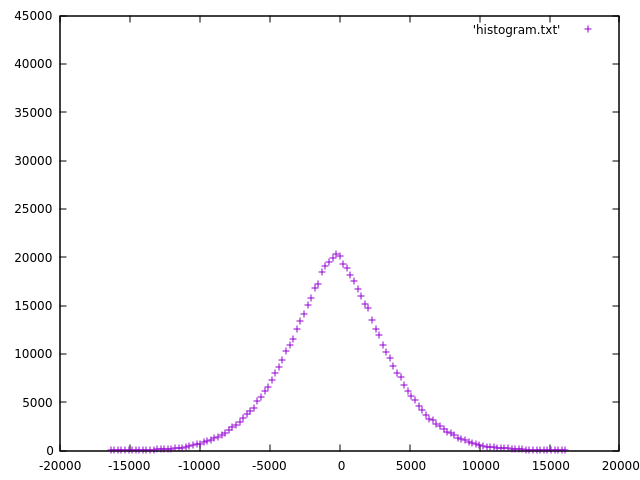
\includegraphics[width=\linewidth]{sample01_8_2.png}
    \caption{{8 bits, 2 reduction}}
    \label{fig:8_2}
  \end{minipage}
  \begin{minipage}{.5\textwidth}
    \centering
    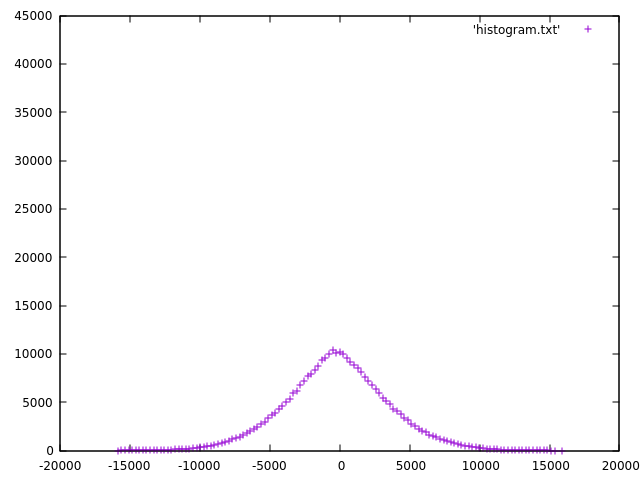
\includegraphics[width=\linewidth]{sample01_8_4.png}
    \caption{{8 bits, 4 reduction}}
    \label{fig:8_4}
  \end{minipage}
\end{figure}

Figures \ref{fig:8_no}, \ref{fig:1_no}, \ref{fig:8_2} and \ref{fig:8_4} depict two different studies, the first two a quantization bit size study and the last two a reduction of the sampling rate study. Figure \ref{fig:8_no} and \ref{fig:1_no} represent the histograms of the music \texttt{sample01} quantized with 8 and 1 bits, respectively and without reduction of the sampling rate. 

A clear takeaway from the figure is that the Figure \ref{fig:8_no} has a lot more frequencies than the Figure \ref{fig:1_no}, which has only two values and the frequency count values in the Figure \ref{fig:1_no} are considerably higher. This behavior is expected since when quantizing a signal we intend to decrease the number of bits necessary to represent each value, discarding the less significant values; for that reason it's expected that when using 1 bit to quantize the signal, there should be 2 resulting values, one in the case the most significant bit is 1 and another if the bit is 0, and between them they should contain all the samples present in the original signal. Theoretically it's possible to encounter $2^{X}$ values/levels, being \texttt{X} the number of bits used to quantize the signal, but in reality this number is not always observed since to original signal can have values that generate every level.

In relation to the Figures \ref{fig:8_2} and \ref{fig:8_4} which represent the reduction sampling rate factor behavior over a mono signal, quantized with 8 bits of the \texttt{sample01} music, it's visible that the higher the reduction the lower the count values become. This directly related to the sampling reduction algorithm implementation, which aggregates as many samples the user indicated, i.e., if the user gave 4 as the reduction factor, the algorithm will then aggregate every 4 samples, creating a 4:1 ratio and decreasing the sampling rate 25\%. This in turn will obviously imply that the number of frequency count values to decrease since there are less values and also due to the aggregation, if there are frequencies very common, those occurrences end up distributed between other frequencies because they were aggregated.   

The C++ scripts mentioned in this chapter all use \texttt{libsndfile}, a C 
library used for reading and writing files containing sampled sound \cite{libsndfile}.
This was proposed on the assignment and allowed us to read and manipulate the 
audio files for more complex tasks.

\newpage
\section*{2. Data Processing}

Once we were capable of visualizing the data, we proceeded to actually doing 
something useful with it.
In this chapter we explain the implementation of the program \texttt{wavquant.cpp},
responsible for reducing the number of bits used to represent each audio sample.
The implementation of the formulas presented on the assignment's description for
the signal-to-noise ratio and the energies of the signals and noises is described
as well, along with the computation of vector quantization codebooks of audio files.

\subsection*{2.1. Uniform Scalar Quantization}

The idea behind a uniform scalar quantization (USQ) is the reduction of bits 
used to represent a signal.
Its usage has an instrinsic tradeoff between signal quality and memory space
required to store the information.
We do not get into much detail regarding the mathematics behind this process, 
but we make available a figure taken from a presentation from the Stanford 
University \cite{stanford} that helps visualizing the outcome of applying the 
USQ to a signal.
Figure \ref{fig:quantization} contains a signal presented in blue and the outcome
of the signal after it is quantized is presented in red. 
The figure also contains the quantization error variation on
the second plot.

\begin{figure}[H]
  \centering
  \begin{minipage}{\textwidth}
    \centering
    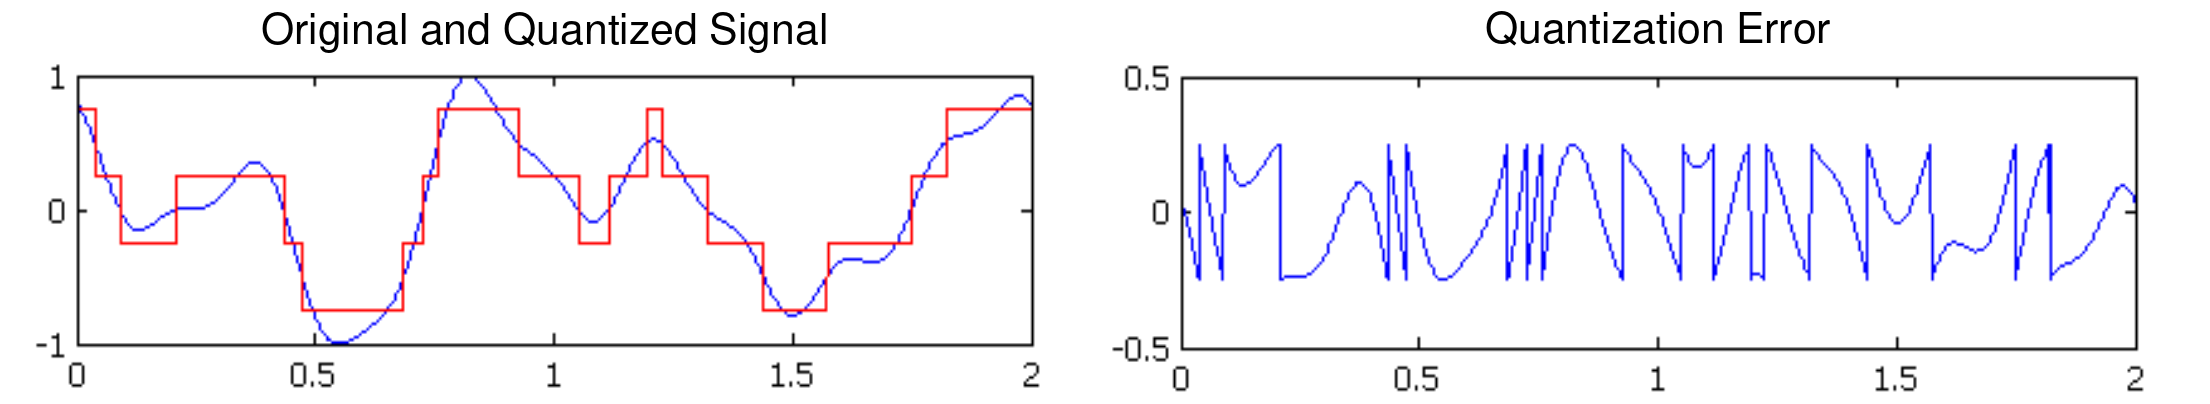
\includegraphics[width=\linewidth]{stanford_quantization_wide.png}
  \end{minipage}%
  \caption{Example of a quantized waveform.}
  \label{fig:quantization}
\end{figure}

It is \texttt{wavquant.cpp} that is responsible for this process.
As we have seen in Section 1.2, the script accepts two optional parameters:
\texttt{quantSize} defines the number of bits to be used to represent the audio 
fragment given as input (ideally, this value should be less than of the original 
source); \texttt{reductFactor} defines the number of times the user would like 
to reduce the total number of values of the audio signal.
This reduction factor works by calculating the average between \texttt{n} values, 
where \texttt{n = reductFactor}, and doing this for all values from the segment.
The result is a signal with \texttt{n} times less values (samples).

\newpage
\subsection*{2.2. Error Calculation}

A signal-to-noise (SNR) ratio compares a level of signal power to a level of 
noise power. 
Higher numbers generally mean a better specification, since there is more useful 
information (the signal) than there is unwanted data (the noise).

In \texttt{wavcb.cpp} we calculate this ratio, along with the maximum absolute 
error per sample. The SNR is defined as stated in equation \ref{eq:1}, taken 
from the assignment's description.

\begin{equation} \label{eq:1}
  SNR = 10 log_{10} \frac{E_{s}}{E_{n}} (dB)
\end{equation}

Here, $E_s$ is the energy of the signal, given by $E_s = \sum_{k} x_k^2$, and
$E_n$ is the energy of the noise, given by $E_n = \sum_{k} (x_k-\bar{x}_k)^2$,
where $x$ is the values from the audio segment.
The maximum error is defined in equation \ref{eq:2}, derived from the noise 
energy equation.

\begin{equation} \label{eq:2}
  error = |x_k-\bar{x}_k| \Leftrightarrow 
  max(error) = max(|x_k-\bar{x}_k|)
\end{equation}

In practice, the error of a quantization tells us how distant from the original
signal is the quantized one.
Figure \ref{fig:quantization} shows an example of how this error looks like.

However, for the following assignment tasks, we determined that the energy of
the noise would be more useful to us.
One way to compare audio fragments would be through the signal-to-noise ratios;
But we found that the only calculations actually required are of the noise 
energies as they work as the distances between two samples.
By focusing on these values, not only do we save processing time, but we are
also able to compare input audio segments to quantization codebooks already 
present in a program to determine the similarity between samples (and 
consequently between segments). These codebooks are explained in this next section.

\subsection*{2.3. Vector Quantization Codebook}
\label{sec:vctQuantCB}

Each song is represented as a sequence of samples, where each sample is a singular frequency if the file is in mono or the frequency of each channel if the file is in stereo that was registered in that exact second. A codebook is an abstract representation of the overall music, and in this context we used the concept of clusters to represent a given number of samples.  The base idea for clustering is the fact that similar data entities should have similar properties and can be aggregated in a group, where data entries that differ significantly from each other, the properties that represent them should be considerably different, implying that they should belong to different groups \cite{clustering}. Dividing the totality of samples present in each song into vectors with X samples and representing them as points in a multidimensional vectorial space, as represented in Figure \ref{fig:pointsEx}, enables the better comprehension of a cluster. Geometrically, clusters can be directly identified by the close grouping of the multidimensional points, since each a axis represent a data property, similar points with similar properties will stay closer to each other. Taking advantage of this natural grouping, clustering algorithms try to find points that represent the several data groups in a viable way, most of the time a middle point of the given group, called \textbf{centroids}.

\begin{figure}[H]
  \centering
  \begin{minipage}{\textwidth}
    \centering
    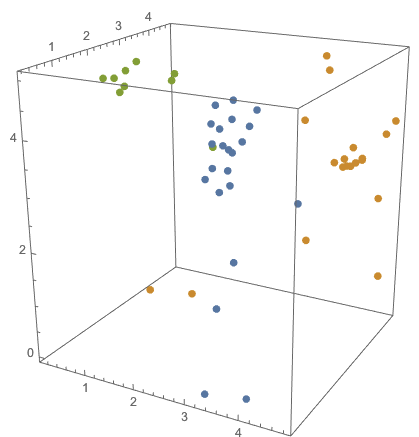
\includegraphics[width=0.5\linewidth]{pointsEx.png}
  \end{minipage}%
  \caption{Example of a quantized waveform.}
  \label{fig:pointsEx}
\end{figure}

For our problem, we used the K-Means Clustering algorithm, probably the most well-known clustering algorithm \cite{clustering}. K-Means is a good approach because it's fast to implement and to execute, since it's only necessary to calculate the distance between a given point and the centroids. 
Our K-Means implementation starts by doing the already mentioned music partition in different blocks/vectors of a given size provided by the user, then the algorithm chooses in a random fashion an a priori given number of centroids. After the pre-processing is done, the main algorithm starts by calculating the closest centroid for each vector, and then updates each centroid by calculating the middle point of the points assigned to that specific centroid, this is repeated as many times as necessary for the error delta, i.e., the error between each iteration to be lower than a given threshold specified by the user. The script \texttt{wavcb} is the implementation of this algorithm and enables the creation of a codebook for a given song, being its interface the following:\\
\texttt{wavcb <inputFile> <blockSize> <overlapFactor> <errorThreshold>\\<numRuns> <outputFile>}\\
Giving a brief explanation of what each parameter means, \textit{inputFile} is the path to the song the user intends to serve as base for the codebook, \textit{blockSize} is the number of samples to be used in the blocks/vectors division, \textit{overlapFactor} is the factor($>$1) that each block will overlap with the previous one, the bigger this percentage is the better the song is represented in the multidimensional space. \textit{errorThreshold} is the maximum error that allowed to exist in last iteration, meaning that the centroids are no longer being adjusted in a significant way, \textit{numRuns} is the number of times the K-Means algorithm will run to find the best local minimum and finally the \textit{outputFile} is the path to the file were the codebook should be stored.\\
Although quite flexible, K-Means has some disadvantages such as the fact that it is necessary to insert the number of centroids to take in consideration, this in many situation is not the best option since the main purpose of using clustering is to get some insights about the data, preferring that the algorithm finds the number of centroids by itself. Another disadvantage is that the K-Means centroids start from a random initial starting position, each means that each run could converge to a local minimum, making each run different from each other.\\
In our implementation we tried to combat the last error by running several times the K-Means algorithm to gain access to several local minimums, being the possible to choose the best one. Even though K-Means is considered a fast clustering algorithm, if given a considerable number of data entries, it's normal it starts to became cumbersome. To combat this aspect we implemented parallelism into the process in two levels, both internal and external which will be explained with further detail in following subsection.

\newpage  
\subsection*{2.4. Codebook Parallel Processing}

As audio files get longer, the number of frames per file increases.
This will lead to the growth of the number of blocks that will be
extracted from it.
Furthermore this blocks can be extracted with overlap among them
which increases even more the total number of blocks.
This high number of blocks, brings computational time implications
since on the step of classification of blocks to the closest
centroids on the K-Means algorithm has to go over all the block and
compare each one to all centroids and get the closest for each block.
To reduce this impact, this step can be parallelized by dividing the
blocks into groups and assigning each group to one thread.
To prevent having to create complex synchronization mechanisms, each
thread stores the association between blocks and the closest
centroids on different data structures and then the main thread is in
charge of reading from those to recalculate the centroids.
% ^^ TODO can be repeating some things from chapter 2.3

% TODO vv might not be true "As mentioned in section "
As mentioned in section 2.3. the K-Means algorithm give us a local
solution for a given centroids' initial position, which means other
and better solutions might exist.
In order to find them, different centroids initializations must be
tested, yet since a K-Means run has high computational cost, several
of them even more computational cost has.
To ease this process, each K-Means run can be assigned to a thread
allowing to execute several runs at the same time.
In terms of implementation it implies some synchronization mechanisms
so the main thread knows when a run was completed and to manipulate
the structure to store the centroids plus associated error calculated
on each run.

\newpage
\section*{3. Automatic Music Identification}

The program \texttt{wavfind.cpp} is the application of the previous scripts on a 
program with a specific purpose.
WAVFind is meant to interpret a mono audio sample and attempt to identify which music 
from a database it belongs to.
In this chapter we discuss our solution, the consequences of varying the 
parameters passed to it and the quality of the results.

\subsection*{3.1. Most Probable Music}

The idea of WAVFind is very similar to the well known mobile app Shazam 
\cite{shazam} - a user plays a sound, the app listens to it, processes it and
determines the most probable music that sound belongs to.
Shazam has a large infrastructure, counting on online real-time music detection,
a nice user interface with access to the smartphone's microphone, and a variety
of other features.
We, on the other hand, focus on the functional end of this idea, implementing
it as a command line program with a limited dataset of known musics and with
the capacity to receive audio segments as input through their respective paths 
on the computer running the command.

To execute this command, one needs to use the following format:

\begingroup
\addtolength\leftmargini{-0.4in}
\begin{quote}
\begin{verbatim}
$ ./wavfind inputFile blockSize overlapFactor codebookDir
\end{verbatim}
\end{quote}
\endgroup

All arguments are mandatory. 
{\it InputFile\/} is the name of the .wav audio whose origin music is to be identified.
{\it BlockSize\/} is the value used as the size of the blocks in which the audio 
segment is split; this value must be the same size used when the codebooks of 
the music dataset were built.
{\it OverlapFactor\/} corresponds to the percentage of each block that is 
overlapped with the following block; this is done to make the program more 
robust in particular situations where, for example, the input audio fragment 
corresponds to the final half of one block and the initial half of the next of a 
codebook.
At last, {\it codebookDir\/} is the path to the directory containing the 
preprocessed codebooks of the music dataset.

The dataflow of the program is as follows:
first, the {\it inputFile\/} is validated and its information is extracted; 
then, it is split into blocks with size according to the parameter {\it blockSize\/}; 
now, for each codebook present in the {\it codebookDir\/}, each segment block 
is compared to each codebook block by calculating the $E_n$ (noise energy) 
between the two;
here, the minimum $E_n$ of each segment block is summed to a cumulative total
that represents the error between the segment and the codebook;
as this cumulative error is calculated for all codebooks, we then check which 
codebook returned the smallest error and assign it as the most similar to the
given audio segment.
This smallest error is determined iteratively - as each codebook is processed, 
we compare its cumulative error to the previous one and keep the smallest.
The identified codebook's is finally printed onto the console (as its name is 
supposed to identify the music it belongs to).

Now, for the program to work properly, there are a few prerequisites.
First of all, the program must have access to the codebook dataset.
The process of creating codebooks is neither trivial nor short-lasting, so to 
have access to the audio dataset is not enough.
Next, the audio segments passed as input files must contain only one signal 
channel (mono).
This restriction reduces the complexity of the comparison process, with the
obvious tradeoff of reducing the quality of the audio.
On the other hand, in a real case scenario (like with Shazam), the user would
usually record audio fragments from external sources such as speakers; so, to 
consider characteristics related to stereo files in the music identification 
process could lead to deceiving the program as the recording could fail in 
distributing the collected information to the proper channels.

\subsection*{3.2. Parameters Variation}

In this section we present some results of executing WAVFind for all datasets.
We also explain some experiences done with variations to the parameters passed
to the command and the respective consequences.

...
BobMarleySong(51,1MB) --- Quantized: 8 bits; 4 reduct factor\\
NoThreads: 40 minutes 6 seconds\\
1\_4: 29 minutes 54 seconds\\
2\_2: 27 minutes 36 seconds\\
2\_1: 31 minutes 25 seconds\\
1\_2: 33 minutes 3 seconds\\
...

\subsection*{3.3. Results Discussion}

...

\newpage
\section*{Conclusions}

After completing the assignment, we drew a few conclusions regarding our 
solutions and the applicability of algorithms such as the K-Means to solving
problems such as music identification.

First of all, ...

Regarding our satisfaction with the delivered code,...

In terms of code organization and readability, we made sure our 
repository was as well structured as possible and our code properly commented
and documented.
The base folder contains a {\it README\/} file for basic instructions and a 
{\it Makefile\/} to make the compilation process easier.
All code is in the {\it src\/} folder and its documentation is accessible, 
with the help of the {\it Makefile\/} and the command "make docs", through
the automatically generated {\it index.html\/} file in the {\it docs\/} 
directory.

\begin{thebibliography}{9}
  \bibliographystyle{Science}

  \bibitem{trab1}
    Armando J. Pinho,
    \textit{AIT: Lab Work no.2},
    University of Aveiro,
    2019/20.
  
  \bibitem{gnuplot}
    H.B. Broeker, G. Clark, L. Hecking and E. Merritt,
    \textit{Gnuplot: graphing utility},
    \url{http://www.gnuplot.info/} ,
    May 2019,
    [accessed in: November 2019].

  \bibitem{libsndfile}
    Free Software Foundation,
    \textit{GLibsndfile API},
    \url{http://www.mega-nerd.com/libsndfile/api.html} ,
    April 2013,
    [accessed in: November 2019].

  \bibitem{stanford}
    Bernd Girod,
    \textit{Image and Video Compression: Quantization},
    \url{https://web.stanford.edu/class/ee398a/handouts/lectures/05-Quantization.pdf} ,
    [accessed in: November 2019].

  \bibitem{shazam}
    Apple Inc.,
    \textit{Shazam for iOS \& Android},
    \url{https://www.shazam.com/apps} ,
    [accessed in: November 2019].

  \bibitem{clustering}
    George Seif,
    \textit{The 5 Clustering Algorithms Data Scientists Need to Know},
    \url{https://towardsdatascience.com/the-5-clustering-algorithms-data-scientists-need-to-know-a36d136ef68} ,
    [accessed in: November 2019].

\end{thebibliography}

\clearpage

\end{document}




















